\section{Method}

To assess whether different robot heights affect the willingness to comply with a robot's request, we designed an interaction with a robot under two conditions: interaction with a Short robot and interaction with a Tall robot (see Figure \ref{fig:MORPHY - A Modular Robotic Platform}). In the experiment, participants performed a cognitive task on a computer, which was presented as the central part of the experiment. After completing the task, participants were informed that the experiment was over. While waiting to receive their credits, the robotic platform entered the room, carrying a tablet with a call to voluntarily fill out a 300-question questionnaire \cite{soto2017next}. This paradigm is based on previous studies that evaluated compliance \cite{boos2022compliance, cialdini1998social, breckler2006social} and with its definition as "A behavior that was requested by another person or group, i.e., an individual acts in some way because someone else has asked them to do so, while they also had the option to refuse" \cite{breckler2006social}. We evaluated whether the robot's height impacted participants' compliance by measuring the number of questions participants agreed to answer in the different conditions. 


 \begin{figure}[t]
     \centering
     \vspace{-0.37cm}
\includegraphics[width=1.2\linewidth]{Figures/Experiment_Room_blueprint-04.png}
     \caption{The experiment room settings and the robots' route.}
     \label{fig:ExperimentSettings}
 \end{figure}


\subsection{Participants}
Forty-four undergraduate students from the university participated in the study (31 females, 13 males; Mean age = 23.6, SD = 2.9). All participants completed an informed consent form and received additional course credits for their participation.

\subsection{Experimental settings}
The experiment was carried out in an experimental room, which included two comfortable armchairs and a small side table next to the armchair where the participant would be seated (see Figure \ref{fig:ExperimentSettings}). The participant used the small table to complete the cognitive task on a laptop brought by the researcher. After completing the task, the participant was asked to return the small table to its original position (verifying that the robot could approach the participant directly). On the far side of the room, there was a camera that allowed the researcher to control the robot's movement using the WoZ technique. We decided on a setup in which all participants were seated to reduce variability related to participants' heights.

 \vspace{0.35cm}

\subsection{Experimental design}
The between-participant experimental design included two conditions: \textit{Short robot} and \textit{Tall robot} (22 \textit{}participants in each condition). The only difference between the conditions was the robot's height (see Figure \ref{fig:Experiment}). The Short robot comprised a base, one body module, and a top module (95 cm in height). The Tall robot comprised a base two body modules and a top module (132 cm in height). To avoid a-priori differences between groups, participants were randomly assigned to the different conditions using a matching technique that balanced gender, tendency for agreeableness \cite{soto2017next}, and Negative Attitudes Toward Robots (NARS) \cite{nomura2006experimental}.


 \begin{figure}[t]
     \centering
      \vspace{0.3cm}
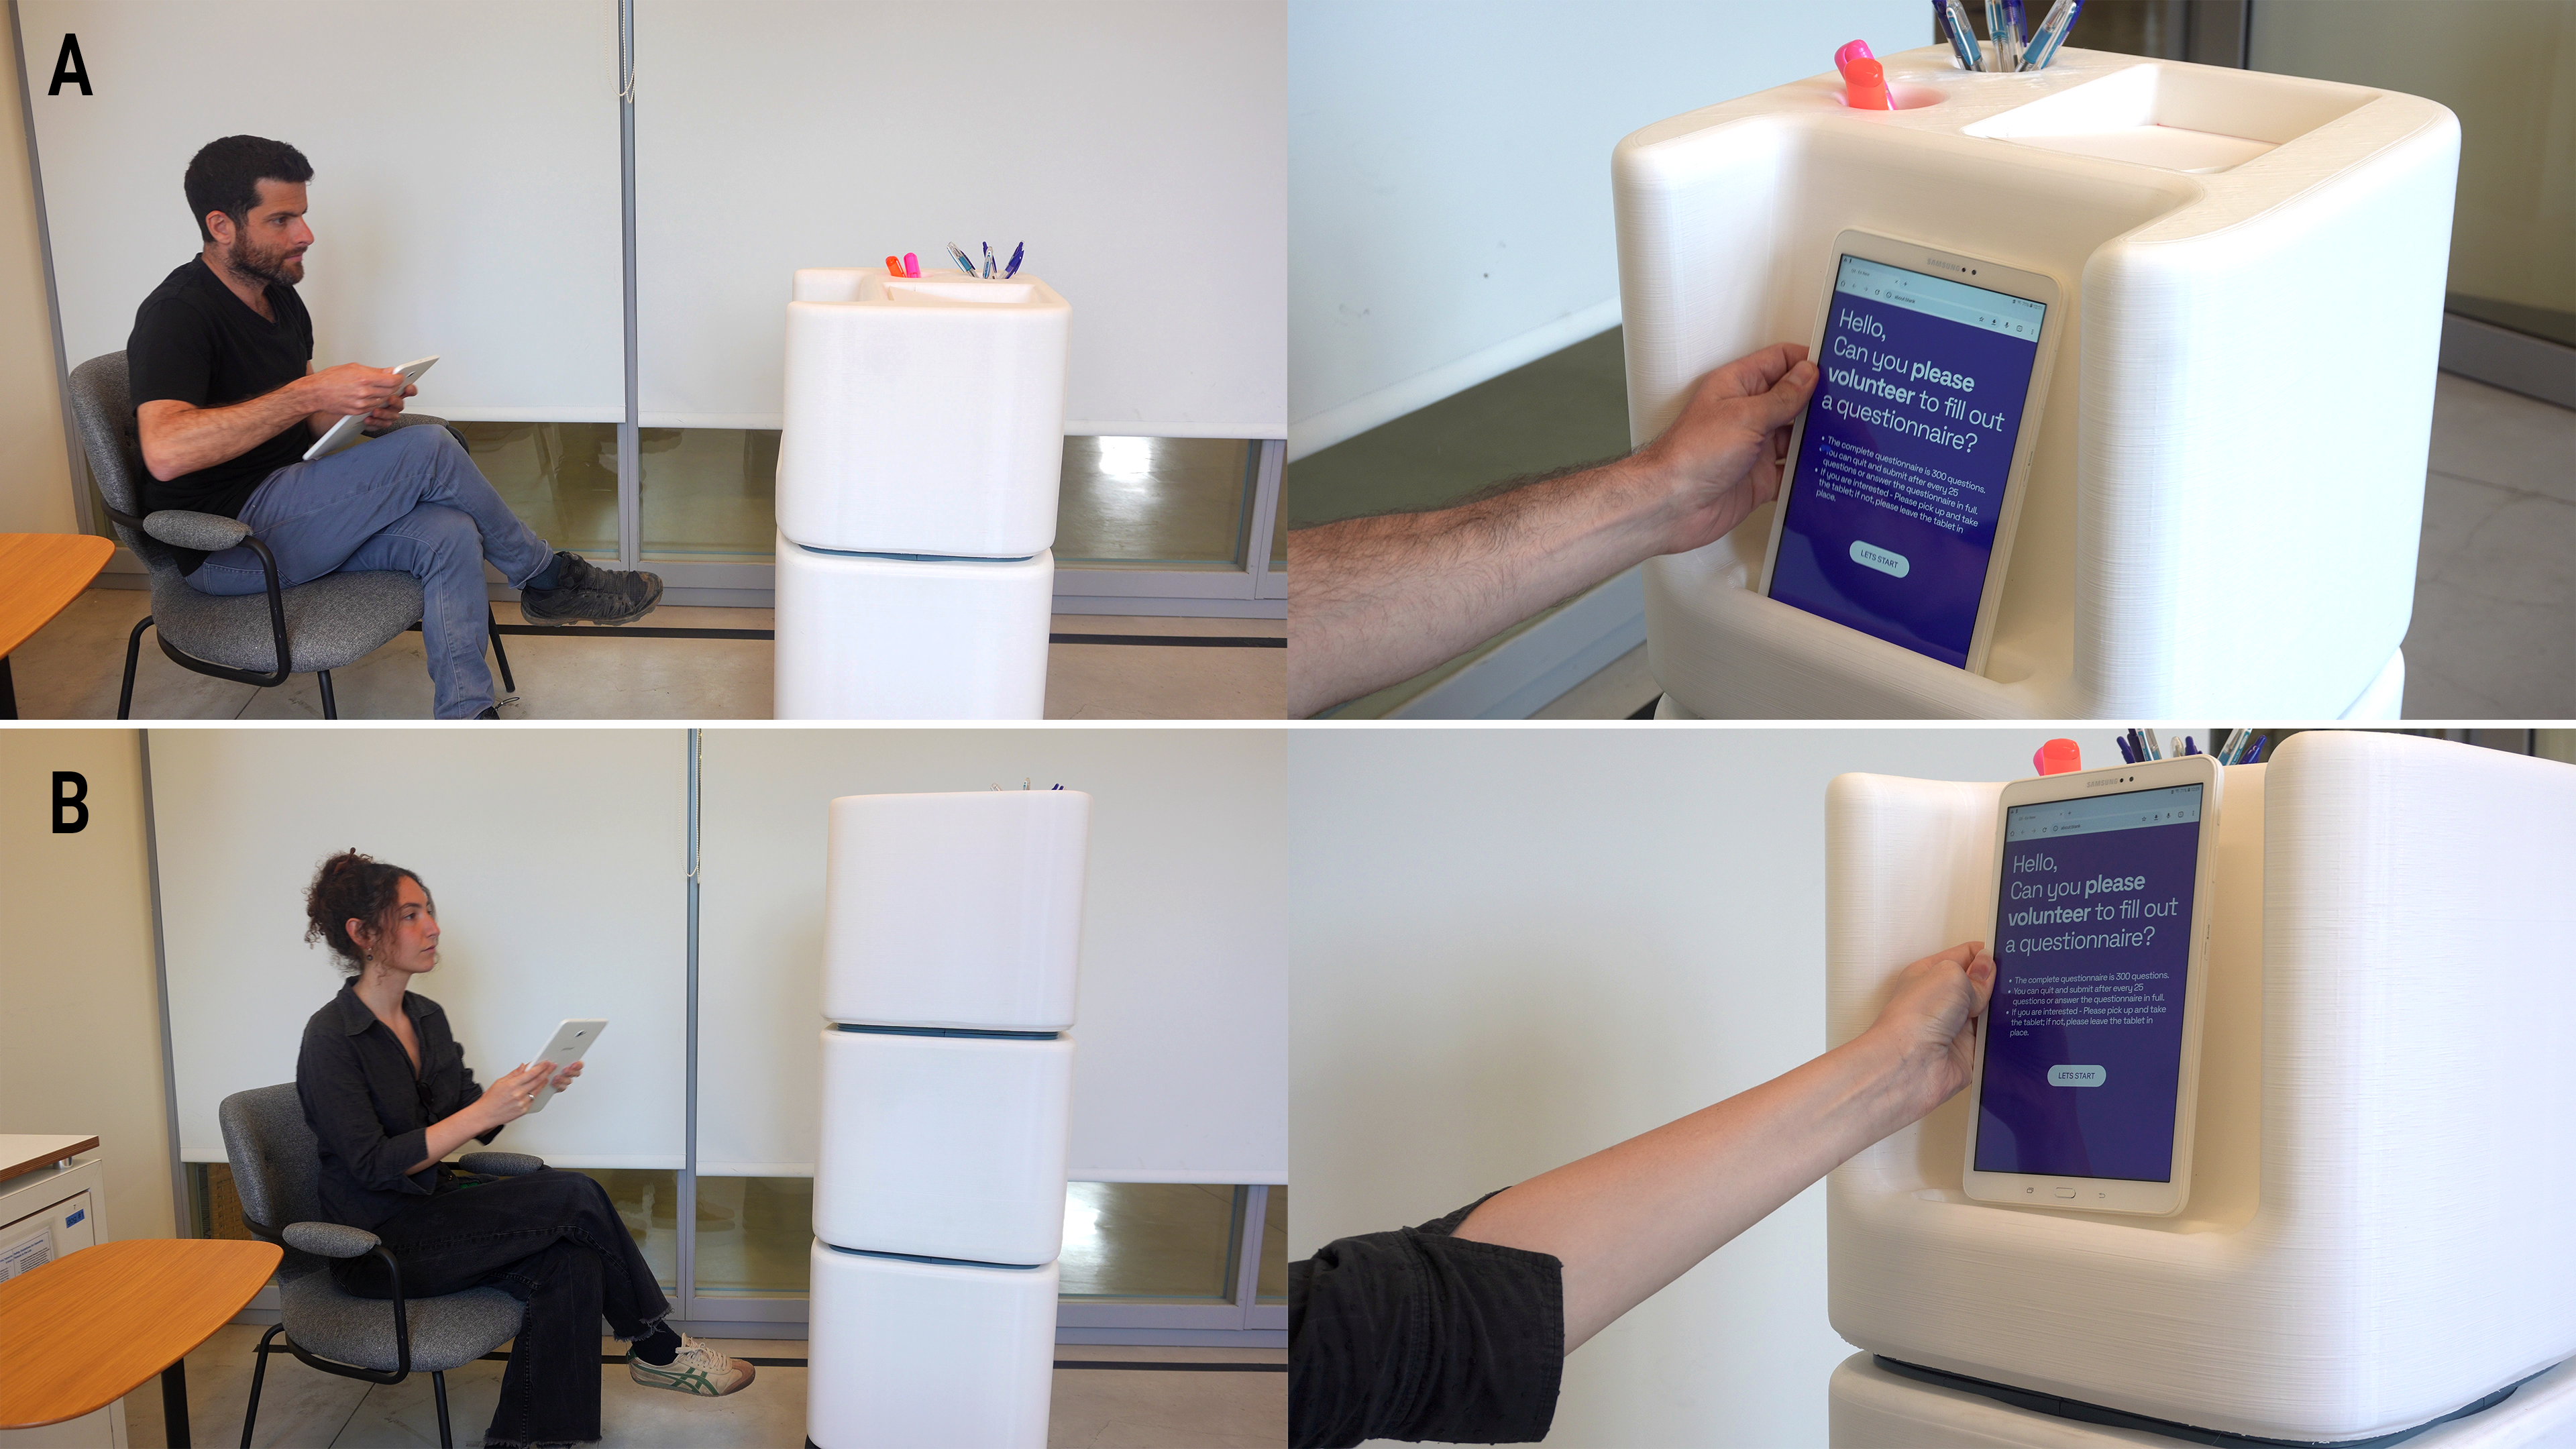
\includegraphics[width=0.9\linewidth]{Figures/MORPHY_RoMan_Experiment-T-and-S.png}
     \caption{A: Short robot condition; B: Tall robot condition.}
     \label{fig:Experiment}
   \end{figure}

    \vspace{0.35cm}

\subsection{Measures}
Quantitative and qualitative measures were utilized to evaluate the impact of the robot's height on participants' level of compliance and their perception of the robot. 

\subsubsection{Compliance} 
We measured participants' compliance by coding whether participants picked up the tablet with the request to answer 300 questions and how many questions they agreed to answer (as after every 25 questions, they had the option to submit their answers and quit or continue to the next page). 

\subsubsection{The Robotic Social Attributes Scale (RoSAS)}
Following the experiment, participants were asked to complete the Robotic Social Attributes Scale (RoSAS) questionnaire to assess their perception of the robot. The questionnaire is a 9-point Likert scale, ranging from 1 ("low") to 9 ("high"), and comprised of three subscales: warmth, competence, and discomfort \cite{carpinella2017robotic}.   

\subsubsection{Semi-structured interviews}
A semi-structured interview was conducted to map participants’ thoughts and attitudes \cite{boyatzis1998transforming}. Questions focused on participants' experience and thoughts about the robot (e.g., “Describe the experience”, "What did you think about the robot?"). 

\subsection{Procedure}
A few days before the experiment, participants received pre-test questionnaires via email, including a Demographic questionnaire, the Agreeableness Trait scale, and the Negative Attitude towards Robots Scale (NARS). Upon arriving at the lab, participants were informed that the experiment was recorded and that they could withdraw from the experiment at any time without penalty. Before entering the experiment room, the researcher informed the participants that since it is a robotics lab, they might encounter robots as those move freely in all parts of the lab. Participants were then guided into the experiment room and were asked to perform a Stroop task (a simple cognitive task that involves naming the ink color of color words) on a laptop placed on a small table next to them. After completing the Stroop test (approximately 10 minutes), the researcher returned to the room and stated that the experiment was completed. The researcher took the laptop and asked the participant to return the side table to its original position (which cleared a path for a robot to approach the participant). The researcher then explained that the credit approval was in the next room and went to get it. During this time, the robot, based on the experimental condition, entered the room with the tablet containing the BFI-2 300-question long questionnaire (see Figure \ref{fig:Tablet}). The robot approached the participant (who was still seated on the armchair) and stopped at 110 cm from the participant. This distance was validated in a short pilot study as a comfortable distance where the participants could easily notice the invitation to volunteer presented on the Tablet. When the participant picked up the tablet, the robot subtly moved backward to give the participants space until they completed the questionnaire. When the participant returned the tablet to its place on the top part of the robot, the robot backed up and drove outside the experiment room. We note that the robot did not use any communication cues besides its movement and the text on the screen. As the robot exited the room, the researcher returned and asked the participant to complete the RoSAS questionnaire and to participate in a semi-structured interview. The researcher then debriefed the participants, gave them their credits, and made sure they left on a positive note. 



 \begin{figure}[b]
     \centering
\includegraphics[width=0.5\linewidth]{Figures/Tablet.png}
     \caption{The tablet with the request to complete a long\\ questionnaire voluntarily.}
     \label{fig:Tablet}
 \end{figure}



